% dsp_cover_image.tex
% 这是一个自包含的 TikZ 绘图脚本
% 它负责定义自己所需的盒子、样式并输出最终图像

% 1. 定义所需的 Savebox (如果未定义)
% --------------------------------------------------
% 将变量定义移到这里,使 .sty 文件保持干净通用
\makeatletter
\@ifundefined{mixedsignalplot}{\newsavebox{\mixedsignalplot}}{}
\@ifundefined{sinesignalplot}{\newsavebox{\sinesignalplot}}{}
\@ifundefined{lpfplot}{\newsavebox{\lpfplot}}{}
\makeatother

% 2. 定义 PGFPlots 样式
% --------------------------------------------------
\pgfplotsset{
    compat=1.18,
    signalplot/.style={
        width=5.5cm, height=3.5cm, 
        hide axis, samples=101, domain=0:12.566,
        enlargelimits=false, ymin=-3.2, ymax=3.2,
    },
    filterplot/.style={
        width=4.5cm, height=3.5cm, 
        samples=51, domain=-5:5, ymin=0, ymax=1.2,
        axis lines=middle, enlargelimits=false, 
        xticklabels={}, yticklabels={},
        xlabel=$\omega$, ylabel=$|H(j\omega)|$,
        every axis x label/.style={at=(current axis.right of origin), anchor=west, font=\small},
        every axis y label/.style={at=(current axis.above origin), anchor=south, font=\small}
    }
}

% 3. 填充 Savebox (预渲染子图)
% --------------------------------------------------
\savebox{\mixedsignalplot}{%
    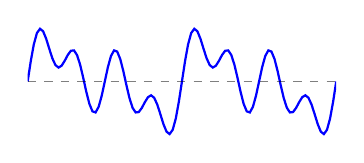
\begin{tikzpicture}
    \begin{axis}[signalplot]
        \addplot [blue, thick] {sin(deg(x)) + sin(deg(2*x)) + sin(deg(4*x))};
        \draw [black, dashed, opacity=0.5] (axis cs:0,0) -- (axis cs:12.566,0);
    \end{axis}
    \end{tikzpicture}%
}

\savebox{\sinesignalplot}{%
    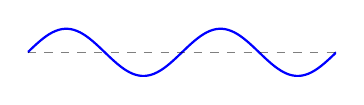
\begin{tikzpicture}
    \begin{axis}[signalplot]
        \addplot [blue, thick] {sin(deg(x))};
        \draw [black, dashed, opacity=0.5] (axis cs:0,0) -- (axis cs:12.566,0);
    \end{axis}
    \end{tikzpicture}%
}

\savebox{\lpfplot}{%
    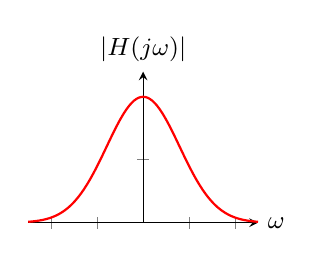
\begin{tikzpicture}
    \begin{axis}[filterplot]
        \addplot [red, thick, smooth] {exp(-0.2*x^2)};
    \end{axis}
    \end{tikzpicture}%
}

% 4. 绘制最终组装图
% --------------------------------------------------
\begin{tikzpicture}[
    plot_node/.style={
        draw, 
        rectangle, 
        inner sep=0pt 
    },
    >=Stealth
  ]
  
  \node (in2) [plot_node] {\usebox{\mixedsignalplot}};
  \node (sys2) [plot_node, right=0.5cm of in2] {\usebox{\lpfplot}};
  \node (out2) [plot_node, right=0.5cm of sys2] {\usebox{\sinesignalplot}};
  
  \draw [->] (in2) -- (sys2);
  \draw [->] (sys2) -- (out2);
  
  \node [
      draw, black,                   
      rounded corners=3pt,           
      fit=(in2) (sys2) (out2), 
      inner sep=10pt                 
  ] {};

\end{tikzpicture}